\chapter{Methodology}

\section{Baseline}
 Our methodology is based on the \textit{"Paint Transformer: Feed Forward Neural Painting with Stroke Prediction"}
by Liu \textit{et al}. We selected Paint Transformer model for two main reasons. 
First, it has a self-learning stroke generation pipeline that does not require 
a pre-existing dataset of strokes, making it easy to train. Second, it uses 
FNNs rather than reinforcement learning, which allows for faster training and 
more stable models.
The Paint Transformer proposed in that paper is already briefly described in 
Chapter 3. The loss function used in that model is described in Section 4.4 
of this chapter. 
The model constructed by Liu \textit{et al} converts an input image into a 
picture-like image drawn by human strokes, but  we aim to address a different 
problem: transforming the content of the input image to match the style of a 
reference image. Specifically, we want to modify the content image such that 
it appears to have been painted with the same brushstrokes as the style image. 

\section{Network Structure}
 Our proposed model utilizes the same Stroke Predictor and Stroke Renderer 
as the baseline model.
A brief description of them was already given in Chapter 3, but we will explain
the Stroke Predictor in more detail.

As mentioned earlier in Chapter 3, the goal of the stroke predictor is to 
predict a set of strokes that don't differ from the reference stroke set. 
At the same time, it is also the goal of it that  to maintain a certain level
of abstraction to simulate the actual painting process.
As shown in Figure \ref{StrokePredictor}, Stroke Predictor uses a Transformer-based model 
that takes in two images: $I_c$ and $I_t$, and generates a stroke set through 
the use of two CNNs and a learnable positional encoding.
$F_c$ and  $F_t$, which are feature maps extracted from CNNs, and 
the encoding are concatenated and flattened as the input to the 
Transformer encoder. The decoder section uses $N$ learnable stroke 
query vectors as input. The output of the decoder consists of two 
branches of fully connected layers: one that predicts the initial 
stroke parameters, and another that predicts stroke confidence 
scores. The confidence scores are used to determine which predicted 
strokes should be plotted on the canvas. 
(For example, in Figure \ref{StrokePredictor}, confidence scores 
for the red, yellow and pink strokes are positive and only those 
are drawn on the canvas.)
During the backward phase of training, the sigmoid function is used 
to compute gradients in order to enable backpropagation.
\begin{figure}[h]
    \centering
    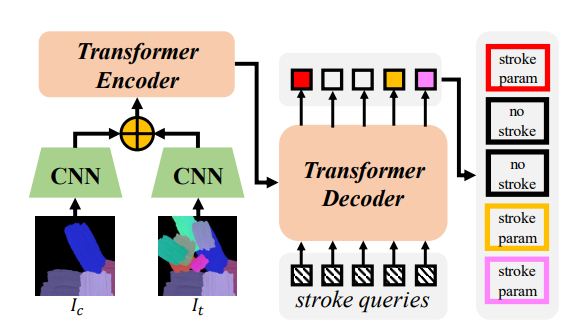
\includegraphics[width=110truemm]{resources/4_methods/StrokePredictor.pdf}
    \caption{
        Image of Stroke Predictor,
        taken from \cite{liu2021paint}.
    }
    \label{StrokePredictor}
\end{figure}

The baseline model takes an input image and generates a version of it that is 
represented as a series of brushstrokes.
However, we wanted to modify this process so that the content of 
the input image is transformed to match the style of a reference 
image, rather than just producing a stroke representation of the 
input image. To achieve this, we made changes to the process 
generating paintings from new images. 
The structure of our proposed model is shown in Figure \ref{Struct_ourmodel}.
The image $I_b$ is created from each base brush image, $G_g^b$ represents the 
gram matrix of $I_b$, and $G_r$ represents the gram matrix of the style 
reference image.

\begin{figure}[h]
    \centering
    \includegraphics[width=135truemm]{resources/4_methods/construct_ourmodel.pdf}
    \caption{
        The structure of our proposed model.
    }
    \label{Struct_ourmodel}
\end{figure}

The baseline provided one brush image, which was used to generate 
strokes by the Paint Transformer model. 
We expanded on this by creating multiple brush images and running 
the Paint Transformer model multiple times to generate pictures 
that depict the content of the input image using each brush image.
We then compared the style of the generated pictures to the style 
of the style reference image and selected the one with the 
smallest loss as the final output image. 

\section{Brush Images}
 Brush images used by the baseline model and created by us are shown in Figure \ref{Brushes}.
(a) is the brush image used by the baseline model, which is a pair of vertical and 
horizontal strokes. 
(b) and (c) are pairs of vertical and horizontal strokes, as was the baseline, 
and subsequent brush images are composed of a single image.
\begin{figure}[h]
    \centering
    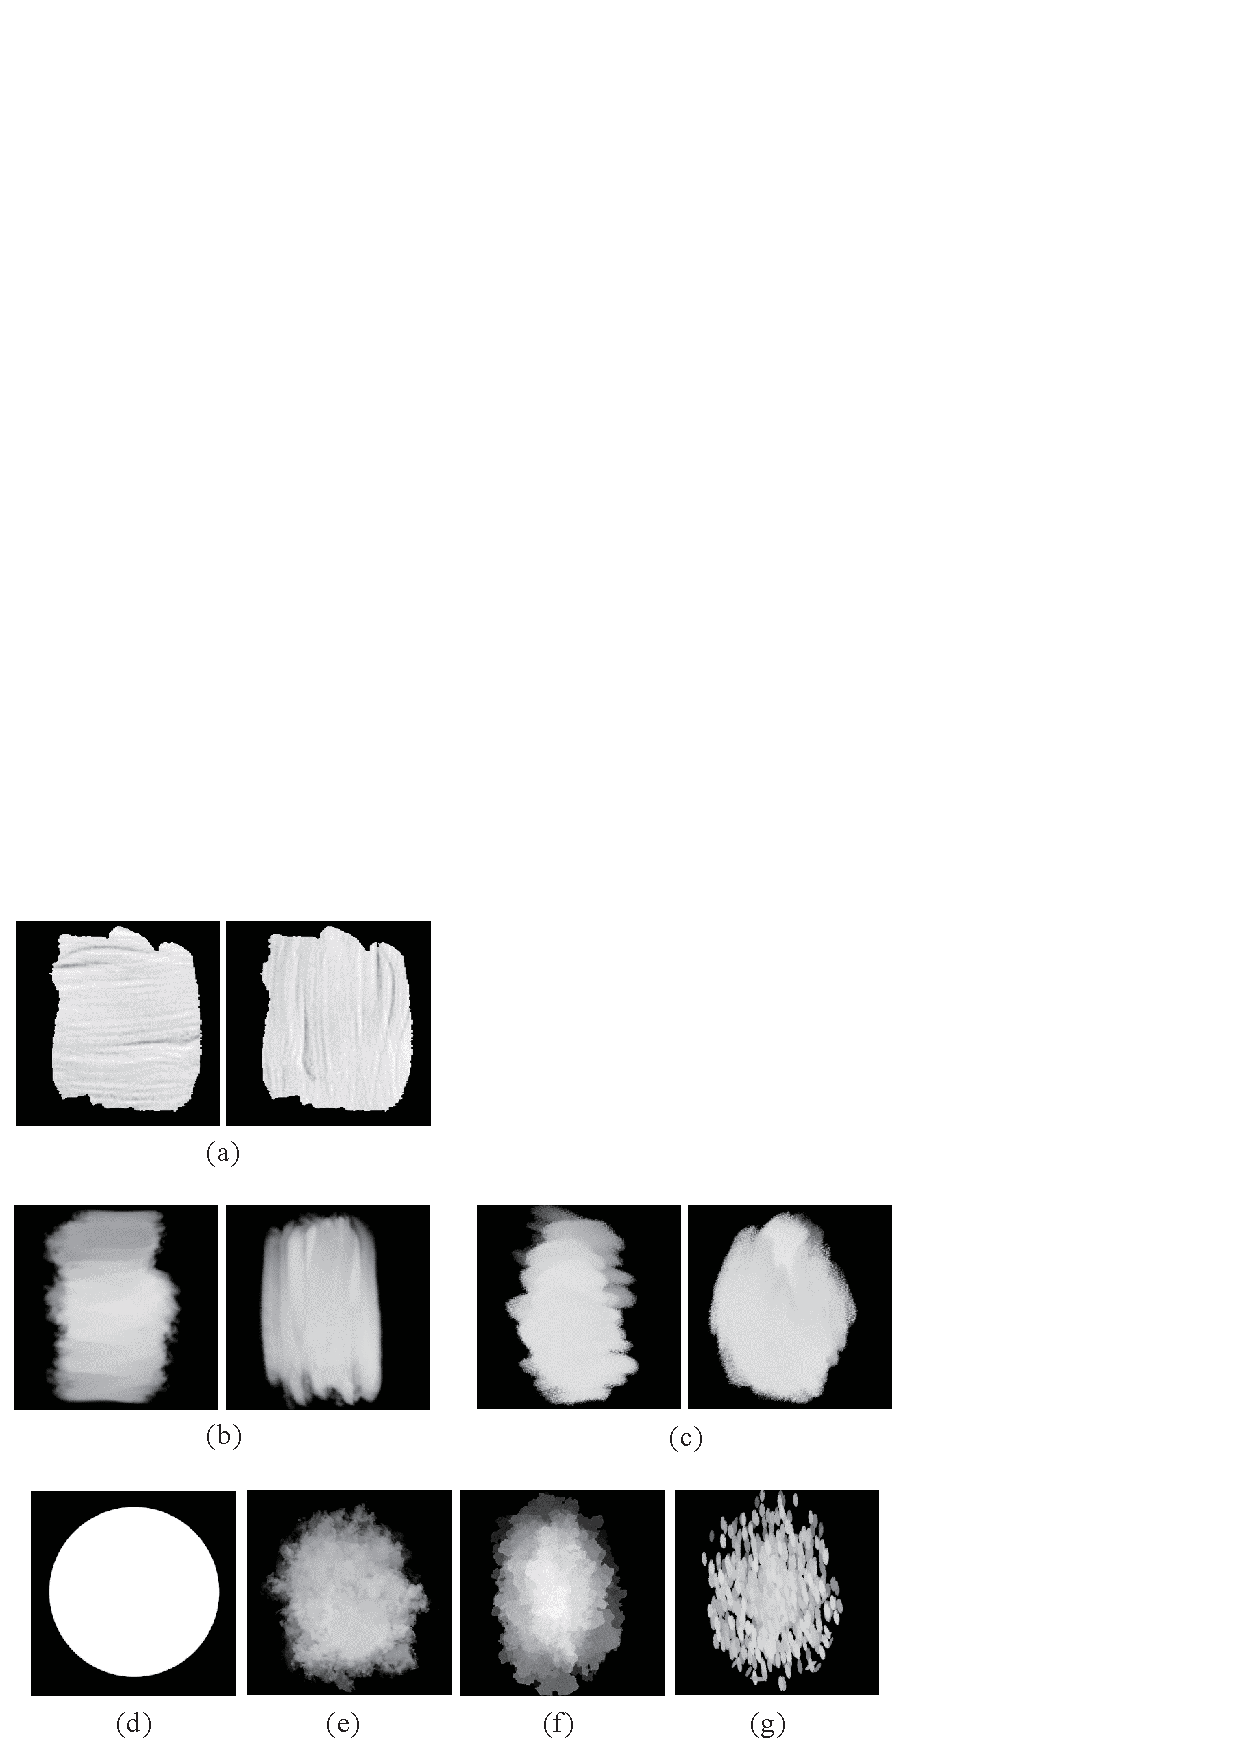
\includegraphics[width=130truemm]{resources/4_methods/brushes.pdf}
    \caption{
        Diversity of brushes developed for more accurate representation of painting effects.
    }
    \label{Brushes}
\end{figure}

\section{Loss Function}
 Since we are using the Paint Transformer proposed by Liu \textit{et al}, 
we also use loss functions proposed by them. However, we did not provide a 
detailed explanation of the loss functions in Chapter 3, so we will discuss 
them first. We will then describe the loss function we propose to measure 
the similarity of brush styles.

Paint Transformer considers loss functions at both the image level and the 
stroke level, and it introduces pixel loss, measurement of differences between
strokes, and stroke loss.
Pixel loss is a measure of the difference between the output image $I_r$ produced 
by the model and the target image $I_t$, which penalized on the image level.
It is expressed as :
\begin{equation}
    \mathcal{L}_{\text {pixel }}=\left\|I_r-I_t\right\|_1
\end{equation}
To measure the difference between two strokes, the L1 distance between two 
strokes, which is a measure of the difference between the parameters of the 
strokes, is defined. (Equation \eqref{L1-distance})
\begin{equation}
    \label{L1-distance}
    \mathcal{D}_{L_1}^{u, v}=\left\|s_u-s_v\right\|_1
\end{equation}
where $s_u$ and $s_v$ denote parameters of strokes u and v respectively. 
However, this measure does not take into account the different scales of 
big and small strokes, so the Wasserstein distance between the strokes is also 
included. The Wasserstein distance is calculated using the Gaussian distributions
of the strokes. 
A rotational rectangular stroke with brush shape parameters ${x, y, w, h, \theta}$
can be regarded as a two-dimensional Gaussian distribution $N(\mu, \sum)$ by the 
Equation \eqref{2D-GD}, and the Wasserstein Distance between two Gaussian 
distributions $N(\mu_u, \sum_u)$ and $N(\mu_v, \sum_v)$ can be expressed as in 
Equation \eqref{Wasserstein}.
\begin{equation}
    \label{2D-GD}
    \begin{aligned} \mu & =(x, y) \\ \boldsymbol{\Sigma}^{\frac{1}{2}} & =\left[\begin{array}{cc}\cos \theta & -\sin \theta \\ \sin \theta & \cos \theta\end{array}\right]\left[\begin{array}{cc}\frac{w}{2} & 0 \\ 0 & \frac{h}{2}\end{array}\right]\left[\begin{array}{cc}\cos \theta & \sin \theta \\ -\sin \theta & \cos \theta\end{array}\right] \\ & =\left[\begin{array}{cc}\frac{w}{2} \cos ^2 \theta+\frac{h}{2} \sin ^2 \theta & \frac{w-h}{2} \cos \theta \sin \theta \\ \frac{w-h}{2} \cos \theta \sin \theta & \frac{w}{2} \sin ^2 \theta+\frac{h}{2} \cos ^2 \theta\end{array}\right]\end{aligned}
\end{equation}
\begin{equation}
    \label{Wasserstein}
    \mathcal{D}_W^{u, v}=\left\|\mu_u-\mu_v\right\|_2^2+\operatorname{Tr}\left(\boldsymbol{\Sigma}_u+\boldsymbol{\Sigma}_v-2\left(\boldsymbol{\Sigma}_u^{\frac{2}{2}} \boldsymbol{\Sigma}_v \boldsymbol{\Sigma}_u^{\frac{1}{2}}\right)^{\frac{1}{2}}\right)
\end{equation}
Additionally, binary cross entropy (Equation \eqref{bce}) is used to match the confidence of the
predicted strokes with their ground truth labels. 
For a predicted stroke $s_u$ with confidence $c_u$ and a target stroke $s_v$ 
with ground truth label $g_v$,  $g_v$ will be equal to 1 if $s_v$ is a valid 
stroke, and $g_v$ will be equal to 0 if $s_v$ is an empty stroke.
\begin{equation}
    \label{bce}
    \mathcal{D}_{b c e}^{u, v}=-\lambda_r \cdot g_v \cdot \log \sigma\left(c_u\right)-\left(1-g_v\right) \cdot \log \left(1-\sigma\left(c_u\right)\right)
\end{equation}
where $\lambda_r$ is a weight term which controls the recall.
For strokes $s_u$ and $s_v$, their cost value is:
\begin{equation}
    M_{u, v}=g_v\left(\mathcal{D}_{L_1}^{u, v}+\mathcal{D}_W^{u, v}+\mathcal{D}_{b c e}^{u, v}\right)
\end{equation}
This function means the matching cost for empty target strokes is always 0.
Therefore, if the optimal permutations of the predicted and target strokes are $X$ and $Y$, 
respectively, the stroke loss function is defined as the sum of these costs, 
weighted by the weight terms  $\lambda_{L1}, \lambda_W$, and $\lambda_{bce}$.
\begin{equation}
    \begin{gathered}
        \mathcal{L}_{\text {stroke }}=\frac{1}{n} \sum_{i=1}^n\left(g_{Y_i}\left(\lambda_{L_1} \mathcal{D}_{L_1}^{X_i Y_i}+\lambda_W \mathcal{D}_W^{X_i Y_i}\right)\right.
        \left.+\lambda_{b c e} \mathcal{D}_{b c e}^{X_i Y_i}\right)
        \end{gathered}
\end{equation}

We adopted the $L1$ loss of the Gram matrix (Equation \eqref{gram}) as a loss function for measuring 
the similarity of brush styles.
By using the Gram matrix, it is possible to consider features over a wide range 
of positions, and we considered it to be effective for dealing with brush styles.


